\section{Solución de Schwarzschild}
\label{sec:solucionSchwarzschild}
\noindent La métrica de Schwarzschild fue la primera solución analítica a las ecuaciones de campo de Einstein. Esta solución comprende el caso mas sencillo posible, el de un objeto esféricamente simétrico y no rotante (Se puede ver la una traducción de la propuesta original en \cite{schwarzschild1999gravitationalfieldmasspoint}, en este texto haremos una derivación inspirada en \cite{eigenchris-2021}).
\begin{itemize}
    \item Tomamos un universo estático y esféricamente simétrico, es decir, un universo que no cambia con el tiempo y que tiene la misma forma en todas las direcciones.
    \item Se usan coordenadas esféricas $(t,r,\theta,\phi)$.
    \item Se Toma una masa puntual M en el origen de coordenadas.
    \item Se asume que no hay materia en el espacio-tiempo, es decir, que el tensor de energía-momento es cero.
    \item lejos de la masa puntual, el espacio-tiempo debe ser plano, es decir, la métrica debe ser la métrica de Minkowski.
\end{itemize}
Al saber que usaremos una simetría esférica, la métrica de Minkowski pasa de las componentes cartesianas a las componentes esféricas, es decir, la métrica de Minkowski en coordenadas esféricas es:
\begin{equation}
    \eta_{\mu \nu}=\left(\begin{array}{cccc}
            -1 & 0 & 0 & 0 \\
            0  & 1 & 0 & 0 \\
            0  & 0 & 1 & 0 \\
            0  & 0 & 0 & 1
        \end{array}\right)=\left(\begin{array}{cccc}
            -1 & 0 & 0     & 0                      \\
            0  & 1 & 0     & 0                      \\
            0  & 0 & r^{2} & 0                      \\
            0  & 0 & 0     & r^{2} \sin ^{2} \theta
        \end{array}\right)
\end{equation}
y
\begin{equation}
    \eta^{\mu \nu}=\left(\begin{array}{cccc}
            -1 & 0 & 0 & 0 \\
            0  & 1 & 0 & 0 \\
            0  & 0 & 1 & 0 \\
            0  & 0 & 0 & 1
        \end{array}\right)=\left(\begin{array}{cccc}
            -1 & 0 & 0               & 0                                \\
            0  & 1 & 0               & 0                                \\
            0  & 0 & \frac{1}{r^{2}} & 0                                \\
            0  & 0 & 0               & \frac{1}{r^{2} \sin ^{2} \theta}
        \end{array}\right),
\end{equation}
Bajo las condiciones de simetría esférica y estática, se imponen los  vectores de Killing $\v{\xi_1 }= \v{e}_t$ ,$\v{\xi_2 }= \v{e}_\theta$ y $\v{\xi_3} = \v{e}_\phi$ .
La implicación de estos Killings 
\begin{align}
\pdi{t}{g_{\mu \nu}} =\pdi{\theta}{g_{\mu \nu}}= \pdi{\phi}{g_{\mu \nu}} = 0 
\end{align}
nos dice por mera eliminación que la métrica solo dependerá de la variable $r$, recordando la situación para una masa puntual en un universo vacío e isotrópico, así que es de esperarse que la métrica no dependa de las coordenadas $\theta$ y $\phi$.


Formalmente, una solución es estática en el tiempo si cumple dos condiciones,
\begin{enumerate}
    \item  Es \textbf{estacionaria}. Implica la invarianza bajo traslaciones en el tiempo, es decir la reversión temporal \( t \to -t \) deja invariante la métrica:
          \[ g_{\mu\nu}(t) = g_{\mu\nu}(-t). \]
Es fácil ver que para términos cruzados mediante las uno formas del elemento de linea
\begin{equation}
\mathbf{dt}\mathbf{dx^i} \neq \mathbf{-dt}\mathbf{dx^i}     
\end{equation}
pero
\begin{equation}
\mathbf{dt}\mathbf{dt} = (\mathbf{-dt})(\mathbf{-dt}) .    
\end{equation}
No hay términos cruzados entre las coordenadas espaciales y temporales, $ g_{ti} = 0 \quad \forall i \in \{r, \theta, \phi\}$ , la métrica en coordenadas de tipo \((t, r, \theta, \phi)\) adopta la forma general. 
\begin{equation}
    g_{\mu \nu} =
    \begin{bmatrix}
        g_{tt} & 0            & 0                & 0              \\
        0      & g_{rr}       & g_{r\theta}      & g_{r\phi}      \\
        0      & g_{\theta r} & g_{\theta\theta} & g_{\theta\phi} \\
        0      & g_{\phi r}   & g_{\phi\theta}   & g_{\phi\phi}
    \end{bmatrix}.
\end{equation}
    \item Es \textbf{irrotacional}.Dadas las simetrías angulares angulares implican que la métrica debe de ser invariante bajo cambios de coordenadas angulares ($\phi \rightarrow  - \phi, \theta \rightarrow  - \theta$).De manera similar con las uno formas se puede ver que

\begin{equation}
\mathbf{dx^i}\mathbf{dx^j} \neq -\mathbf{dx^i}\mathbf{dx^j}, \quad (i \neq j ) . 
\end{equation}

Y los componentes cruzados de la métrica deben ser cero, haciendo la métrica diagonal. 
\begin{equation}
    g_{\mu \nu} =
    \begin{bmatrix}
        g_{tt} & 0            & 0                & 0              \\
        0      & g_{rr}       &   0    &  0  \\
        0      & 0 & g_{\theta\theta} &0 \\
        0      &  0  & 0 & g_{\phi\phi}
    \end{bmatrix}.
\end{equation}
\end{enumerate}



Debido a que estamos usando una simetría esférica y que la métrica es diagonal,la métrica de la sub variedad debe ser asintótica a la descrita por una esfera de radio $r$ \footnote{La aparición de un termino $(\sin \theta)^2$, no contradice que la métrica dependa solo de $r$, ya que esta función es una parte fija de la estructura de la 2-esfera}, y le podemos multiplicar una función  escalar radial $C(r)$.
\begin{equation}
    \begin{array}{ll}
        g_{\theta \theta} & g_{\theta \phi} \\
        g_{\phi \theta}   & g_{\phi \phi}
    \end{array} = \left[\begin{array}{cc}
            C(r) r^2 & 0                       \\
            0        & C(r) r^2(\sin \theta)^2
        \end{array}\right].
\end{equation}


Los componentes desconocidos serán entonces 3 funciones dependientes de $r$
\begin{equation}
    \left[\begin{array}{cccc}
            -A(r) & 0    & 0        & 0                       \\
            0     & B(r) & 0        & 0                       \\
            0     & 0    & C(r) r^2 & 0                       \\
            0     & 0    & 0        & C(r) r^2(\sin \theta)^2
        \end{array}\right].
        \label{eq:genericMetric}
\end{equation}
Mediante cambio de variable 

\begin{equation}
    \tilde{r}=\sqrt{C(r)}  r,
\end{equation}
que permite escribir la métrica \ref{eq:genericMetric} como 
\begin{equation}
    \left[\begin{array}{cccc}
            -A(\tilde{r}) & 0    & 0        & 0                       \\
            0     & B(\tilde{r}) & 0        & 0                       \\
            0     & 0    & \tilde{r}^2 & 0                       \\
            0     & 0    & 0        & \tilde{r}^2(\sin \theta)^2
        \end{array}\right].
        \label{eq:genericmetric2}
\end{equation}
Aprovechando el carácter tensorial que hace la métrica sea valida independiente de la elección de coordenadas  $\tilde{r}$ la escribiré como $r$, esto se hace sin perdida de la interpretación de las coordenadas esféricas puesto que $\tilde{r}$ es una función monótona creciente de $r$.


La forma de proceder va a ser  calcular los Christoffel para después llegar al tensor de Ricci que debe de cumplir las ecuaciones de vacío (\ref{vacuumFieldEquations})
\begin{equation*}
    g_{\mu \nu} \rightarrow \Gamma_{\mu \nu}^\sigma \rightarrow R_{\mu \nu}.
\end{equation*}
Los símbolos de Christoffel los obtenemos a partir de 

\begin{equation}
    \Gamma_{\mu \nu}^\sigma=\frac{1}{2} g^{\sigma \rho}\left(\partial_\nu g_{\mu \rho}+\partial_\mu g_{\nu \rho}-\partial_\rho g_{\mu \nu}\right).
\end{equation}
El calculo se realizo con el programa del anexo \ref{chap:programa_christoffel} y se encontraron los Christoffel no cero 
\begin{equation}
\begin{aligned}
    &\Gamma_{01}^0=\Gamma_{10}^0=\frac{1}{2} \frac{1}{A}\left(\partial_r A\right),\\ 
    &\Gamma_{00}^1=\frac{1}{2} \frac{1}{B}\left(\partial_r A\right),\\
    &\Gamma_{11}^1=\frac{1}{B}\left(\partial_r B\right),\\
    &\Gamma_{22}^1=-\frac{r}{B},\\
    &\Gamma_{33}^1=-\frac{r(\sin \theta)^2}{B},\\
    &\Gamma_{12}^2=\Gamma_{21}^2=\Gamma_{13}^3=\Gamma_{31}^3=\frac{1}{r},\\
    &\Gamma_{33}^2=-\sin \theta \cos \theta,\\
    &\Gamma_{23}^3=\Gamma_{32}^3=\cot \theta
\end{aligned}
\end{equation}

Para calcular el tensor de Ricci $R_{\mu \nu}$ se obtiene contrayendo el tensor de Riemann,
\begin{equation}
    R_{\mu \nu}=R_{\mu \alpha \nu}^\alpha=\partial_\alpha \Gamma_{\mu \nu}^\alpha-\partial_\nu \Gamma_{\mu \alpha}^\alpha+\Gamma_{\alpha \lambda}^\alpha \Gamma_{\mu \nu}^\lambda-\Gamma_{\nu \lambda}^\alpha \Gamma_{\mu \alpha}^\lambda .
    \label{eq:ricci_tensor}
\end{equation}
El calculo se hizo con el programa del anexo \ref{chap:programa_ricci}, con un poco de refinamiento manual, se obtuvieron los componentes del tensor de Ricci 

\begin{equation}
    \begin{array}{l}
    R_{00}=2 r A B A^{\prime \prime}-r A A^{\prime} B^{\prime}+4 A B A^{\prime}-r B\left(A^{\prime}\right)^2=0 ,\\
    R_{11}=-2 r A B A^{\prime \prime}+r B\left(A^{\prime}\right)^2+r A A^{\prime} B^{\prime}+4 A^2 B^{\prime}=0, \\
    R_{22}=-2 A B+2 A B^2-r A^{\prime} B+r A B^{\prime}=0.
    \end{array}
    \end{equation}
Si sumamos los componentes $R_{00} + R_{11} = 0 $

\begin{equation}
    \begin{aligned}
        4 A B A^{\prime} + 4 A^2 B^{\prime} = 0 \\
        B A^{\prime}+A B^{\prime}=0 \\
        \partial_r(A B)=0 \\
        \Rightarrow A B=K
    \end{aligned}
\end{equation}
donde \( K \) es una constante de integración. Para determinar \( K \), consideramos el límite cuando \( r \to \infty \):
\begin{equation}
    \begin{aligned}
         & \lim_{ r \to \infty} A(r) = 1, \\
         & \lim_{ r \to \infty} B(r) =   1.
    \end{aligned}
\end{equation}
$A(r)$ y $B(r)$ son funciones que tienden a 1 cuando \( r \to \infty \), ya que la métrica en este caso debe de ser asintótica  a Minkowski . Por lo tanto, \( K = 1 \) y

\begin{equation}
    \Rightarrow B(r)=\frac{1}{A(r)} \text { para todo } r, \quad  B^{\prime}=\partial_r\left(A^{-1}\right)=-\frac{A^{\prime}}{A^2}.
\end{equation}
Con esta información es posible sustituir \( B(r) \) en la ecuación \( R_{22} = 0 \)
\begin{equation}
    \begin{aligned}
         & R_{22}=-2 A B+2 A B^2-r A^{\prime} B+r A B^{\prime}   = 0                                                           \\
         &-2 A \frac{1}{A}+2 A\left(\frac{1}{A}\right)^2-r A^{\prime} \frac{1}{A}+r A\left(-\frac{A^{\prime}}{A^2}\right)=0\\
         & -2 + 2 \frac{1}{A}-\frac{r A^{\prime}}{A}- \frac{r A^{\prime}}{A}=0 \\
            & -2 + \frac{2}{A} - \frac{2r A^{\prime}}{A}=0 \\
            &\Rightarrow  A^{\prime} + \frac{A}{r}=\frac{1}{r}.
    \end{aligned}
    \label{eq:ricci22}
\end{equation}
Resolviendo la ecuación anterior por factor integrante,
\begin{equation}
    \begin{aligned}
        A &= e^{- \int 1/r d r} \left[\int \left(\frac{1}{r}e^{\int 1/r dr } \right)dr - k\right]\\
        &= e^{- \ln r} \left[\int \frac{1}{r} e^{\ln r} dr   - k\right] \\
        &=\frac{1}{r}\left[\int dr - k\right]\\
        &= 1 - \frac{k}{r}. \\
    \end{aligned}
\end{equation}
Inmediatamente se desvela que $B=\frac{1}{1 - \frac{k}{r}}  $,por lo que la métrica queda como:
\begin{equation}
    g_{\mu \nu} =\left[\begin{array}{cccc}
        -\left(1-\frac{k}{r}\right) & 0                                & 0    & 0                   \\
            0             & \left(1-\frac{k}{r}\right)^{-1} & 0    & 0                   \\
            0             & 0                                & r^2 & 0                   \\
            0             & 0                                & 0    & r^2(\sin \theta)^2
        \end{array}\right]
\end{equation}
Por ultimo debemos de tomar la aproximación de campo débil en el limite newtoniano para obtener la constante de integración \( k \) (véase \cite[148-149]{ryder-2009} )
\begin{equation}
    g_{\mu \nu} =  \eta_{\mu \nu}+ h_{\mu \nu} .
\end{equation}
Centrémonos en el componente \( g_{tt} \) donde \( h_{tt} = -\frac{-2 \mathbf{\Phi}}{c^2}  = \frac{2MG}{rc^2}\) 
\begin{equation}
    g_{tt} = -1 + \frac{k}{r} = \eta_{tt} + h_{tt} = -1 + \frac{2GM}{rc^2}
\end{equation}
Donde $k = \frac{2GM}{c^2}$.
\begin{definition}{Metrica de Schwarzschild}{}
La métrica de Schwarzschild es una solución exacta a las ecuaciones de campo de Einstein en el vacío, que describe el campo gravitacional de un objeto esféricamente simétrico y no rotante. La métrica se expresa como:
\begin{equation}
    g_{\mu \nu}=\left(\begin{array}{cccc}
                -1+\frac{2 G M}{r c^2} & 0                                       & 0   & 0                  \\
                0                      & \left(1-\frac{2 G M}{r c^2}\right)^{-1} & 0   & 0                  \\
                0                      & 0                                       & r^2 & 0                  \\
                0                      & 0                                       & 0   & r^2 \sin ^2 \theta
            \end{array}\right)
            \label{eq:schwarzschild_metric}
\end{equation}
\end{definition}
Observe que la métrica  \ref{eq:schwarzschild_metric} diverge ``aparentemente'' cuando \( r = 2GM/c^2 \equiv r_s\), este punto se conoce como \textbf{radio de Schwarzschild},  y se denomina entonces que cuando el radio del cuerpo es menor a  $r_s $,la region que corresponde a $r<r_s $ la métrica describe la geometría de un agujero negro, y $r_s$ es la  frontera del horizonte de eventos del agujero negro. También es usual encontrase con este punto definido como $r_s = 2GM/c^2 =2m $, la ultima notación ($2m$) se encuentra cuando se trabaja con unidades naturales pero aquí  nos referiremos a  $m = GM/c^2$ como un simple cambio de variable.  

\subsection{Geodésicas en Schwarzschild tipo  nulas}

\noindent El movimiento de los cuerpos y de la luz en el espacio-tiempo de Schwarzschild está dado por la ecuación geodésica
\begin{equation}
    \frac{\mathrm{d}^2 x^\mu}{\mathrm{d} \lambda^2}+\Gamma^\mu{ }_{\nu \rho} \frac{\mathrm{~d} x^\nu}{\mathrm{d} \lambda} \frac{\mathrm{~d} x^\rho}{\mathrm{d} \lambda}=0.
    \label{eq:geodesic}
\end{equation}
Con $x^0 = ct$, $x^1 = r$, $x^2 = \theta$, $x^3 = \phi$ y $\lambda$ es un parámetro afín.

Los símbolos de Christoffel no cero son
\begin{equation}
        \begin{array}{l}
        \Gamma^0{ }_{10}=\Gamma^0{ }_{01}=\dfrac{G M}{c^2 r\left(r - \dfrac{2 G M}{c^2}\right)},                                                                                                                       \\
        \Gamma^1{ }_{11}=-\dfrac{G M}{c^2 r\left(r - \dfrac{2 G M}{c^2}\right)}, \quad \Gamma^1{ }_{22}=-\left(r - \dfrac{2 G M}{c^2}\right), \quad \Gamma^1{ }_{33}=-\left(r - \dfrac{2 G M}{c^2}\right) \sin \theta, \\
        \Gamma^2{ }_{12}=\Gamma^2{ }_{21}=\Gamma^3{ }_{13}=\Gamma^3{ }_{31}=\dfrac{1}{r}, \quad \Gamma^2{ }_{33}=-\sin \theta \cos \theta,                                                                             \\
        \Gamma^3{ }_{23}=\Gamma^3{ }_{32}=\cot \theta.
    \end{array}
\end{equation}

Particularmente nos interesa el caso de geodésicas nulas, es decir, aquellas que describen la trayectoria de la luz en el espacio-tiempo, por lo que se toma la ecuación genérica de geodésica, y se impone la condición $ds^2 = 0$  . Además se considera $\theta=\pi/2$ y $\phi=0$, para una simplificación de los cálculos  (Si se desea ver las demás trayectorias solo hay que remplazar los valores en la ecuación \ref{eq:geodesic}).

Considere  la ecuación geodésica con $\mu=0$ es

\begin{equation}    
    \frac{\mathrm{d}^2 t}{\mathrm{d} \lambda^2}+\dfrac{2 G M}{c^2 r\left(r - \dfrac{2 G M}{c^2}\right)} \frac{\mathrm{d} t}{\mathrm{d} \lambda} \frac{\mathrm{d} r}{\mathrm{d} \lambda}=0
\end{equation}

ó
\begin{equation}
    \frac{\mathrm{d}}{\mathrm{~d} \lambda}\left[\left(1-\dfrac{2 G M}{c^2 r}\right) \frac{\mathrm{d} t}{\mathrm{~d} \lambda}\right]=0,
\end{equation}
lo cual se integra para dar
\begin{equation}
    \left(1-\dfrac{2 G M}{c^2 r}\right) \frac{\mathrm{d} t}{\mathrm{~d} \lambda}=b=\text { const. }
\end{equation}
Tomando elemento de linea ``light-like'' $ds^2 = 0$ que es la condición que describe precisamente a la luz 
\begin{equation}
    \begin{aligned}
        \mathrm{d} s^2 & =g_{\mu \nu} \mathrm{d} x^\mu \mathrm{d} x^\nu                                                                      \\
                       & =-\left(1-\dfrac{2 G M}{r c^2}\right)c^2 \mathrm{d} t^2+\left(1-\dfrac{2 G M}{r c^2}\right)^{-1} \mathrm{d} r^2 = 0
    \end{aligned}
\end{equation}
manipulando la relación de la geodésica tipo luz
\begin{equation}
    \left(1-\frac{2 G M}{r c^2}\right)^{-1} \frac{dt}{d\lambda}  = b \rightarrow  \left(\frac{dt}{d\lambda}\right)^2 = b^2 \left(1-\frac{2 G M}{r c^2}\right)^{-2},
\end{equation}
que implica  entonces
\begin{equation}
    \frac{d r }{d \lambda}= \pm cb.
\end{equation}
Podemos relacionar $r$ con $t$  de la siguiente manera
\begin{equation}
    \frac{\frac{dr}{d\lambda}}{\frac{dt}{d\lambda}} =   \frac{dr}{dt} =  \frac{\pm cb }{ b \left(1-\frac{2 G M}{r c^2}\right)^{-1}} = \pm c \left(1-\frac{2 G M}{r c^2}\right).
\end{equation}
Resolviendo esta ultima ecuación
\begin{equation}
    ct = \pm \left(r + \frac{2 G M}{c^2} \ln \abs{r -\frac{2 G M}{c^2} } + k \right)
\end{equation}
o en términos de el radio de Schwarzschild $r_s = \frac{2 G M}{c^2}$
\begin{equation}
    ct = \pm \left(r + r_s \ln\abs{r - r_s} + k \right)
    \label{eq:lightRaysSchwarzschild}
\end{equation}
donde el signo $+$ es para geodésicas salientes y el signo $-$ es para geodésicas entrantes.
\begin{figure}[H]
    \begin{small}
        \begin{center}
            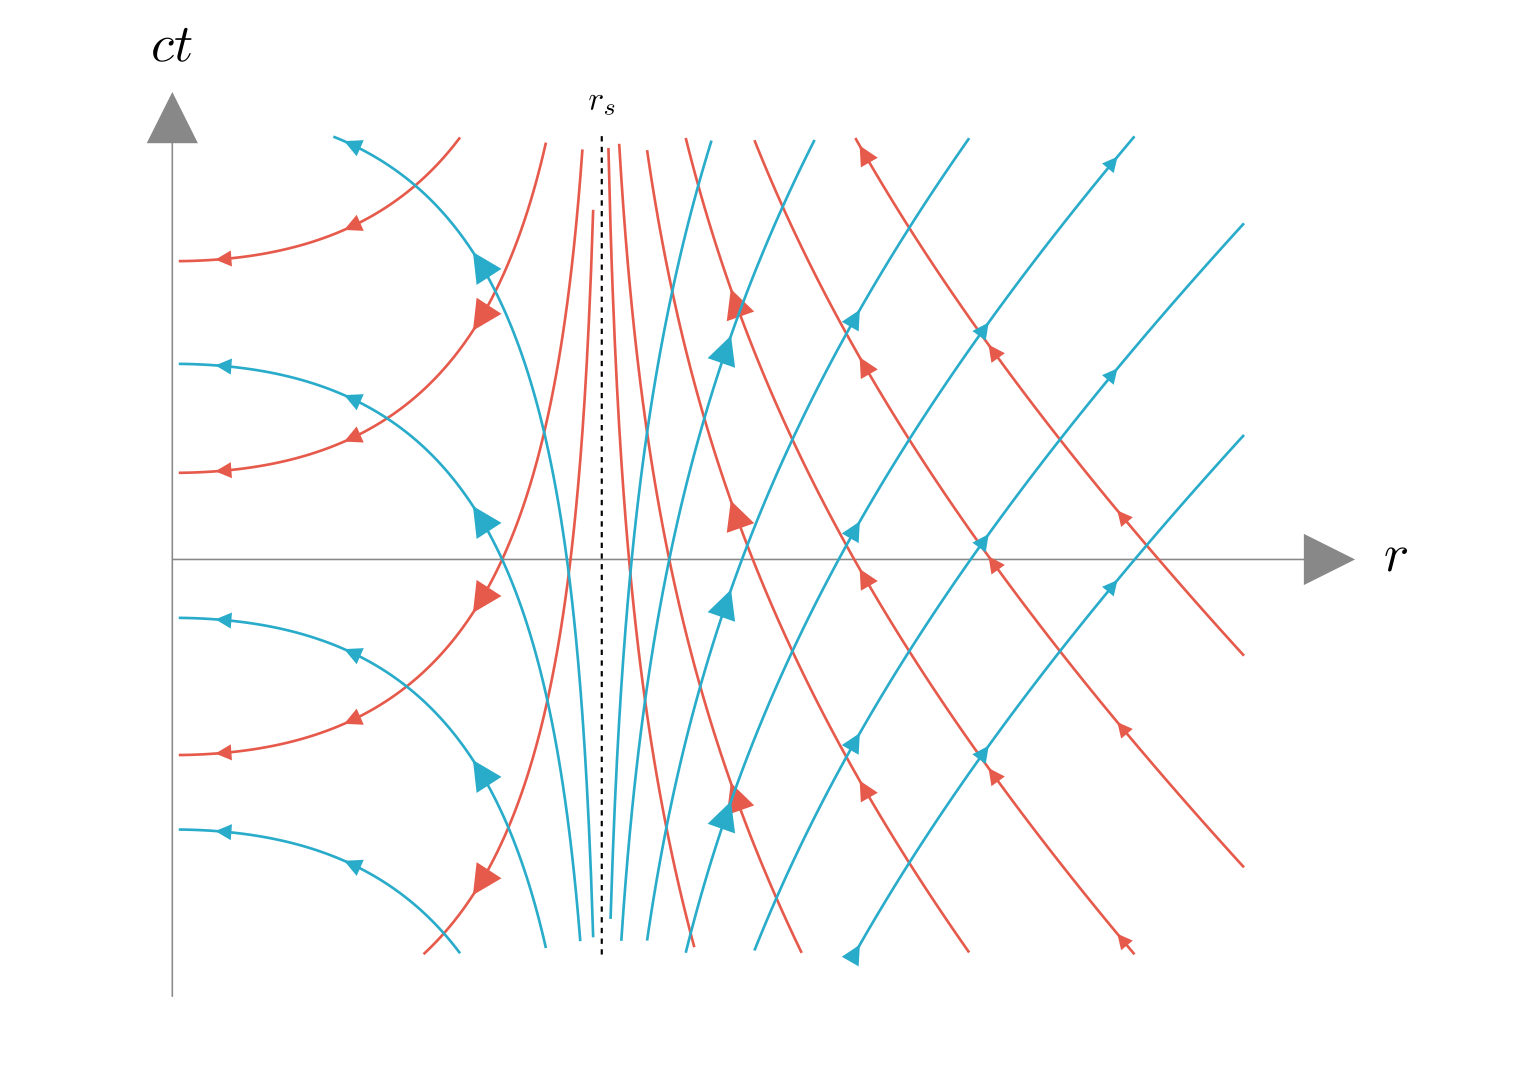
\includegraphics[width=0.99\textwidth]{AgujerosNegros/Schwarzschild/media/images/rayos_Luz_Schwarzschild_ManimCE_v0.19.0.png}
        \end{center}
        \caption{Gráfica $ct,r $ representando las trayectorias tipo luz, las salientes, son representadas de color azul y las entrantes en color rojo }
        \label{fig:lightraysSchwarzschild}
    \end{small}
\end{figure}

\subsection{Coordenadas Eddington-Finkelstein}
Las coordenadas de Eddington-Finkelstein son un sistema de coordenadas para la solución de Schwarzschild cuya idea principal es usar las trayectorias de la luz (geodésicas nulas radiales) para definir las coordenadas temporal y radial.
Partimos de la trayectoria de luz \ref{eq:lightRaysSchwarzschild} que esta en términos de la coordenada radial \( r \) y el tiempo \( ct \) e introducimos la nueva coordenada \( c\tilde{t} \), normalmente llamada coordenada temporal avanzada
\begin{equation}
        c\tilde{t}  = ct + r_s \ln \left| \frac{r}{r_s} - 1 \right|,      \Rightarrow 
        ct         = c\tilde{t} - r_s \ln \left| \frac{r}{r_s} - 1 \right|.
    \label{eq:ctVariables}
\end{equation}
Combinando la nueva coordenada con la ecuación de las geodésicas entrantes (\( - \)) en (\ref{eq:lightRaysSchwarzschild})
\begin{equation}
    c\tilde{t} - r_s \ln \left| \frac{r}{r_s} - 1 \right| = -r - r_s \ln \left| \frac{r}{r_s} - 1 \right| + k,
\end{equation}
simplificando 
\begin{equation}
    c\tilde{t} = -r + k  .
\label{eq:ctVariablesIn}
\end{equation}
Si tomamos el signo \( + \) de la ecuación de luz saliente (\( + \)) en (\ref{eq:lightRaysSchwarzschild}), y hacemos el mismo procedimiento de introducir el cambio de variable (\ref{eq:ctVariables}) para las geodésicas salientes
\begin{equation}
    c\tilde{t} = r + 2 r_s \ln \left| \frac{r}{r_s} - 1 \right| + k.
\end{equation}

\begin{figure}[H]
    \begin{small}
        \begin{center}
            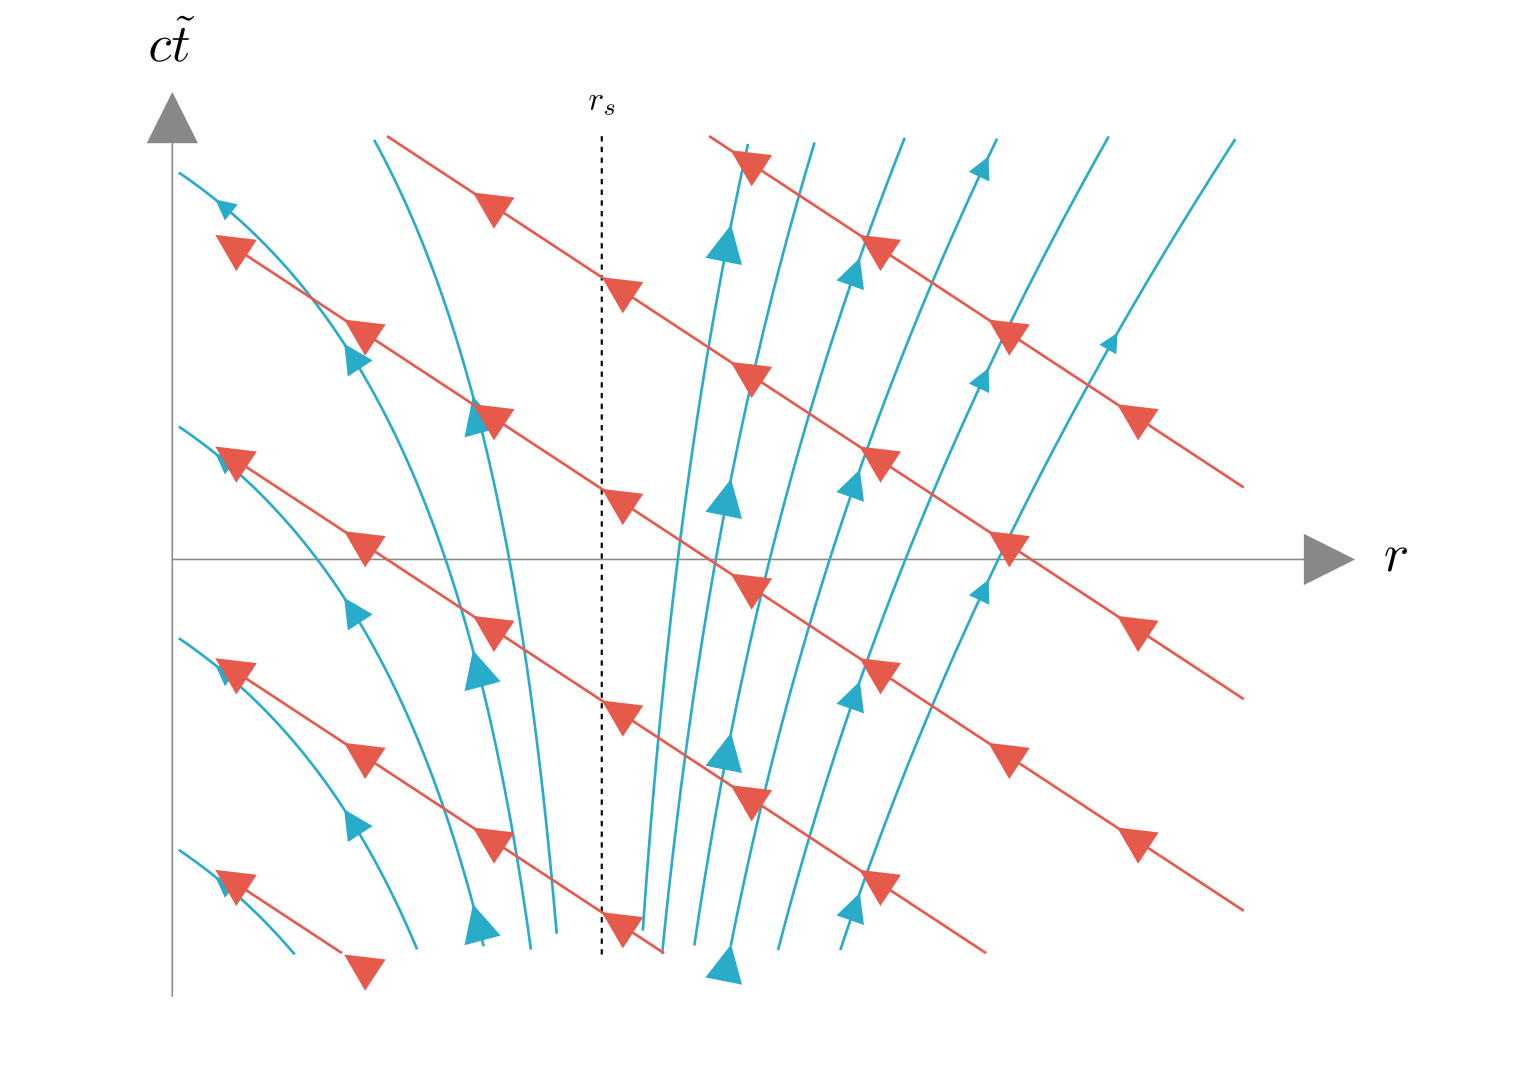
\includegraphics[width=0.95\textwidth]{AgujerosNegros/Schwarzschild/media/images/EddingtonFinkelsteinIngoingLight_ManimCE_v0.19.0.png}
        \end{center}
        \caption{Geodésicas nulas entrantes y salientes en coordenadas avanzadas}
        \label{fig:EddingtonFinkelsteinInLight}
    \end{small}
\end{figure}
La idea base de las coordenadas de Eddington-Finkelstein es que las geodésicas nulas nos permiten definir un nuevo sistema de coordenadas que no diverja en el horizonte de eventos(aquí hay que notar que aunque la coordenada avanzada $c\tilde{t}$ nos dejo hacer que las geodésicas tipo luz pasen sin problema su definición sigue presentando una divergencia en $r_s$), ya que estas pueden cruzarle sin problemas como se ve en la figura \ref{fig:EddingtonFinkelsteinInLight}.Al montar la nueva coordenada \( v \) sobre las geodésicas entrantes tipo luz con valores constantes \ref{eq:ctVariablesIn} haciendo la asignación a la nueva coordenada como  $v = k$, se define

\begin{equation}
    \begin{aligned}
        v &= c\tilde{t} + r ,\\
        v  & = ct + r + r_s \ln \left| \frac{r}{r_s} - 1 \right|, \\
        ct & = v - r - r_s \ln \left| \frac{r}{r_s} - 1 \right|.
    \end{aligned}
\end{equation}
Una vez que hemos hecho la asignación para los rayos entrantes, se calcula cual es la trayectoria de los rayos salientes usando la ecuación anterior y la ecuación(\ref {eq:lightRaysSchwarzschild})(+),
\begin{equation}
    \begin{aligned}
        ct = v - r - r_s \ln \left| \frac{r}{r_s} - 1 \right|= r + r_s \ln \left| \frac{r}{r_s} - 1 \right| + k, \\
        v = 2 \left(r + r_s \ln \left| \frac{r}{r_s} - 1 \right|\right) +k.
    \end{aligned}
\end{equation}

\begin{figure}[H]
    \begin{small}
        \begin{center}
            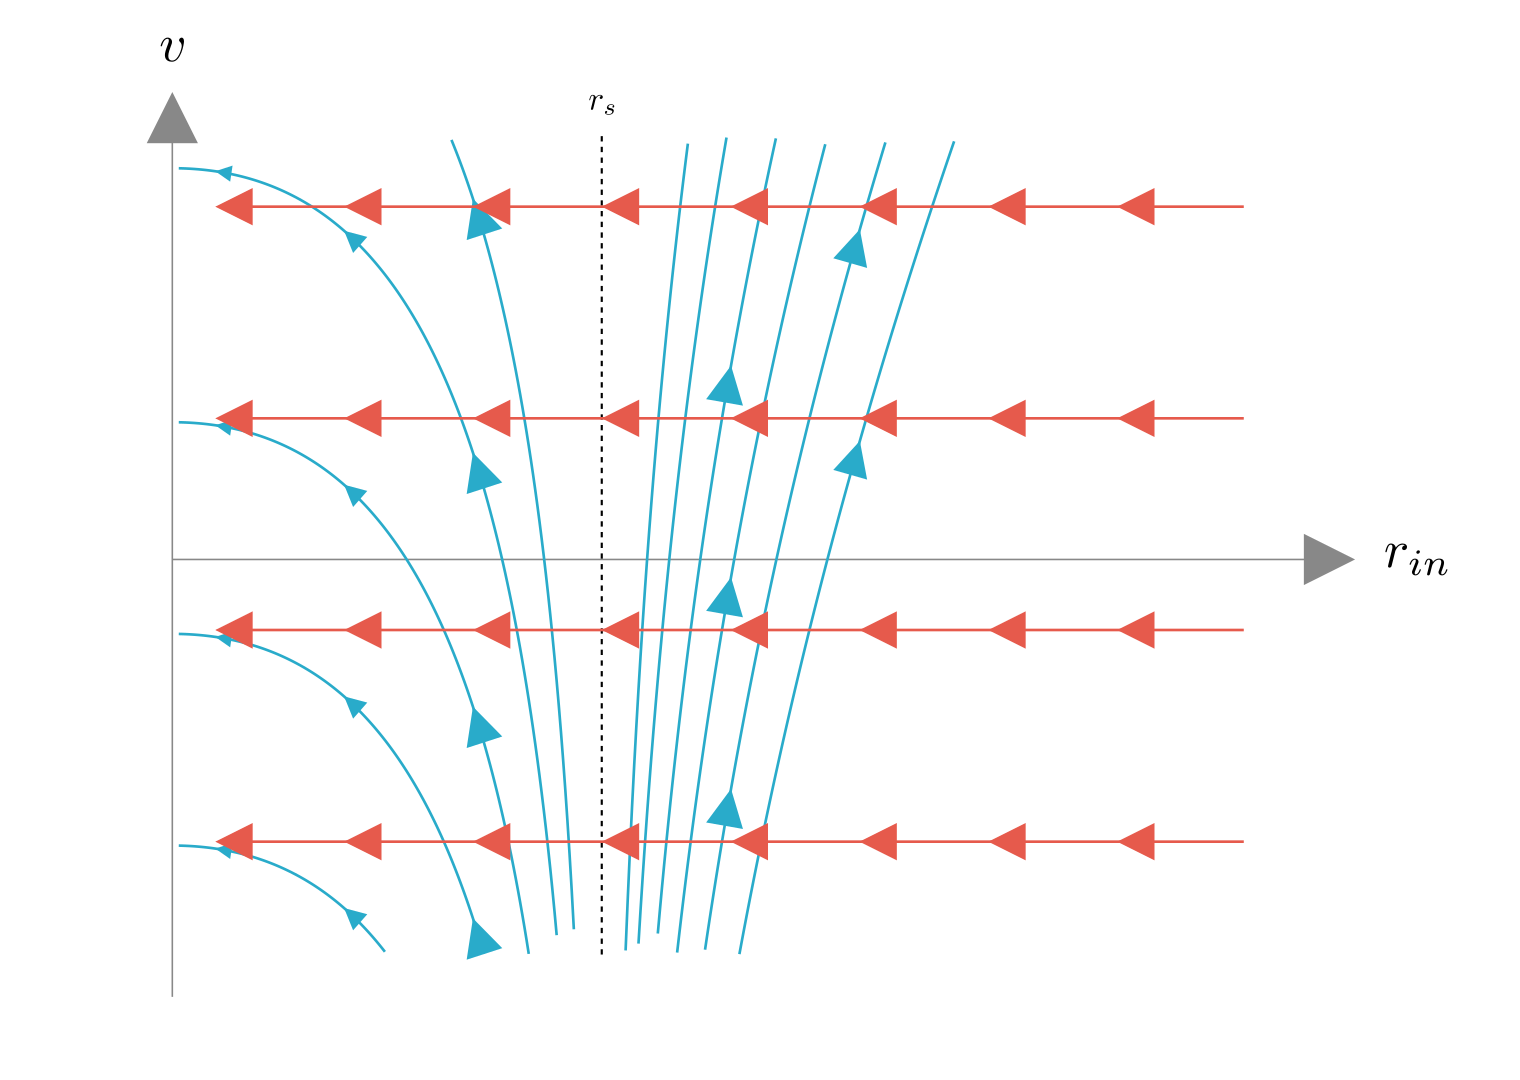
\includegraphics[width=0.95\textwidth]{AgujerosNegros/Schwarzschild/media/images/EddingtonFinkelsteinVR_ManimCE_v0.19.0.png}
        \end{center}
        \caption{Diagrama de los rayos de luz en coordenadas de Eddington-Finkelstein. Las líneas azules representan los rayos entrantes y las rojas los salientes. Las nuevas coordenadas no ortogonales \(v\) y \(r_{\text{in}}\) están definidas en función de las originales \(v = ct + r + r_s \log \left| \frac{r}{r_s} - 1 \right|\) y \(r_{\text{in}} = r\) .}
    \end{small}
\end{figure}

\subsubsection{Métrica de Schwarzschild en coordenadas de Eddington-Finkelstein}
La métrica se obtiene expresando los vectores base \( e_v \) y \( e_{r_{\text{in}}} \) en términos de las bases originales \( e_{ct} \) y \( e_r \). 
Los vectores base transforman como sigue
\begin{equation}
    \begin{aligned}
        \v{e_v}               & = \frac{\partial ct}{\partial v} \v{e_{ct}} + \frac{\partial r}{\partial v} \v{e_r} = \v{e_{ct}},                                                            \\
        \v{e_{r_{\text{in}}} }& = \frac{\partial ct}{\partial r_{\text{in}}} \v{e_{ct}} + \frac{\partial r}{\partial r_{\text{in}}} \v{e_r} = -\frac{1}{1 - \frac{r_s}{r}} \v{e_{ct}} + \v{e_r}.
    \end{aligned}
\end{equation}

Los componentes de la métrica \( g_{\mu\nu} = \v{e_\mu} \cdot \v{e_\nu} \) son:

\begin{equation}
    \begin{aligned}
        g_{vv}          & = \v{e_v} \cdot \v{e_v} = -\left(1 - \frac{r_s}{r}\right), \\
        g_{vr} = g_{rv} & = \v{e_v} \cdot \v{e_{r_{\text{in}}}} = 1,                 \\
        g_{rr}          & = \v{e_{r_{\text{in}}}} \cdot \v{e_{r_{\text{in}}}} = 0.
    \end{aligned}
\end{equation}
Por lo tanto, la métrica en coordenadas entrantes de Eddington-Finkelstein es 
\begin{equation}
    ds^2 = -\left(1 - \frac{r_s}{r}\right) dv^2 + 2 dv dr + r^2 d\Omega^2,
\end{equation}
nótese que bajo este nuevo esquema de coordenadas la métrica no se indetermina en el horizonte de eventos \( r = r_s \).  
\subsubsection{Coordenadas salientes de Eddington-Finkelstein}
De forma análoga a como hicimos el cambio de coordenadas para tener los rayos de luz entrantes con valores constantes, para geodésicas nulas salientes (\(+\)) de la ecuación (\ref{eq:lightRaysSchwarzschild}) introducimos la coordenada \( u \):
\begin{equation}
        u  = ct - r - r_s \log \left| \frac{r}{r_s} - 1 \right|.
\end{equation}
Para rayos salientes (\(+\)) de forma completamente análoga al procedimiento anterior \(u = k\).
Y para los entrantes (\(-\)):
\begin{equation}
    \begin{aligned}
        u + r + r_s \log \left| \frac{r}{r_s} - 1 \right| = -r - r_s \log \left| \frac{r}{r_s} - 1 \right| + k, \\
        u = -2\left(r + r_s \log \left| \frac{r}{r_s} - 1 \right|  \right) +k.
    \end{aligned}
\end{equation}
\begin{figure}[H] 
    \centering 
    \begin{subfigure}{0.48\textwidth} 
        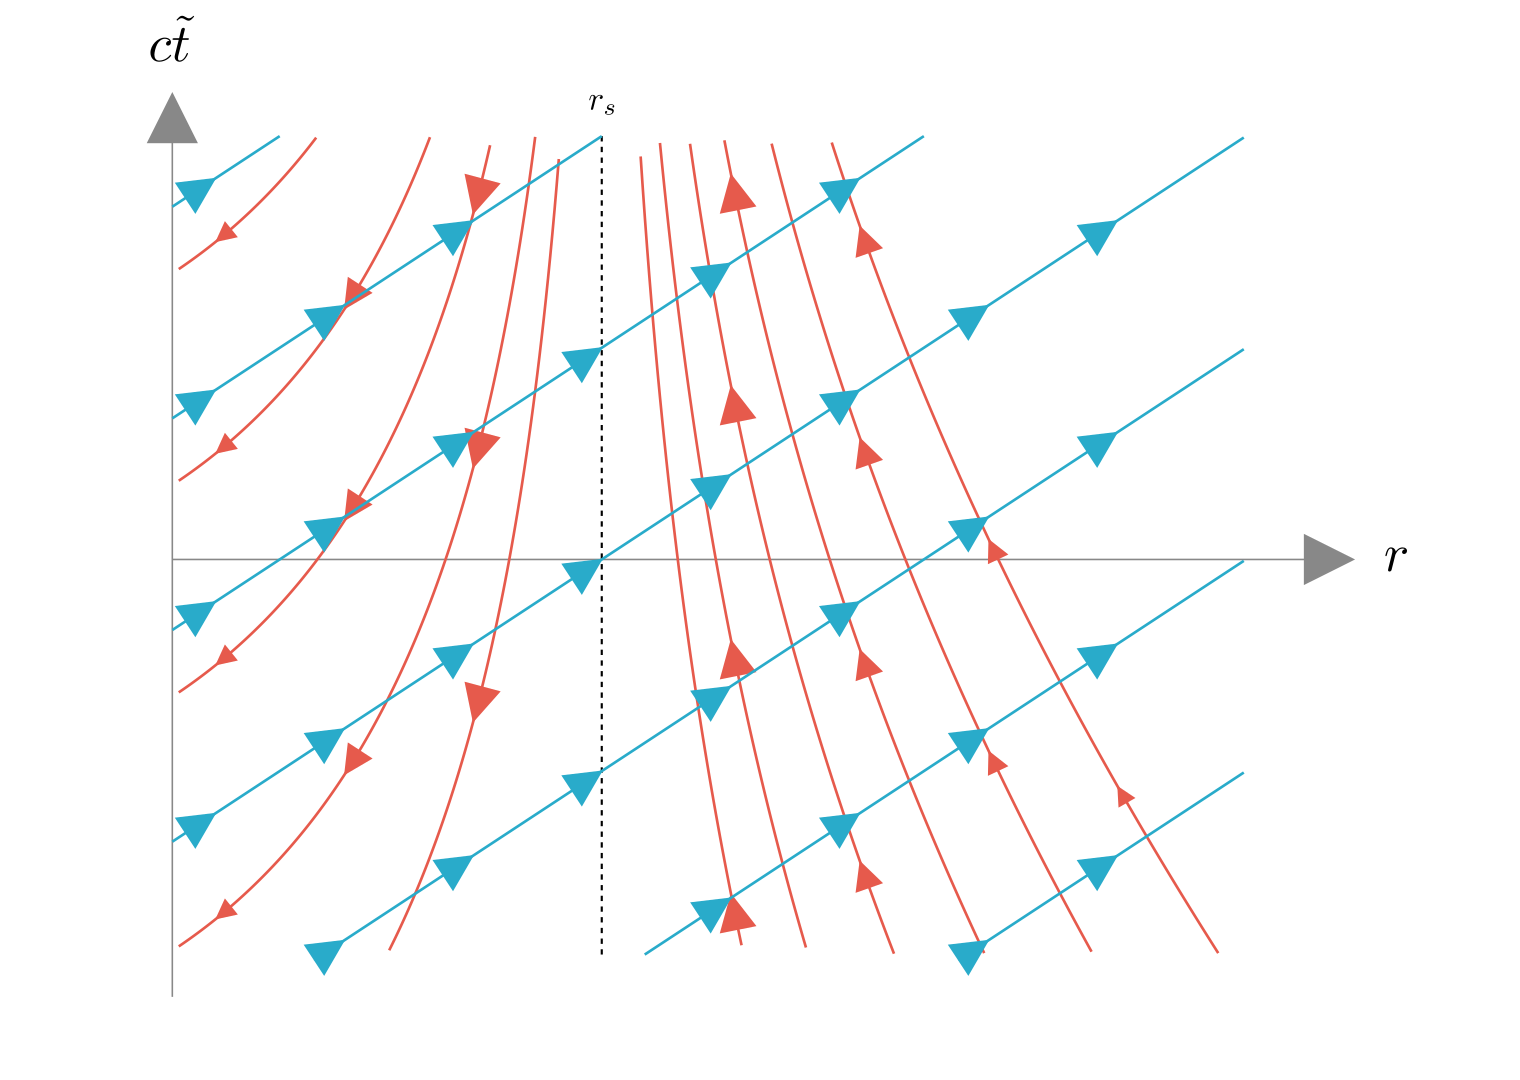
\includegraphics[width=\linewidth]{AgujerosNegros/Schwarzschild/media/images/EddingtonFinkelsteinOutgoingLight_ManimCE_v0.19.0.png}
        \caption{Rayos de luz con coordenada temporal atrasada $ c \tilde{t} = ct - r_s \ln \left| \frac{r}{r_s} - 1 \right|$.}
    \end{subfigure}
    \hfill 
    \begin{subfigure}{0.48\textwidth} 
        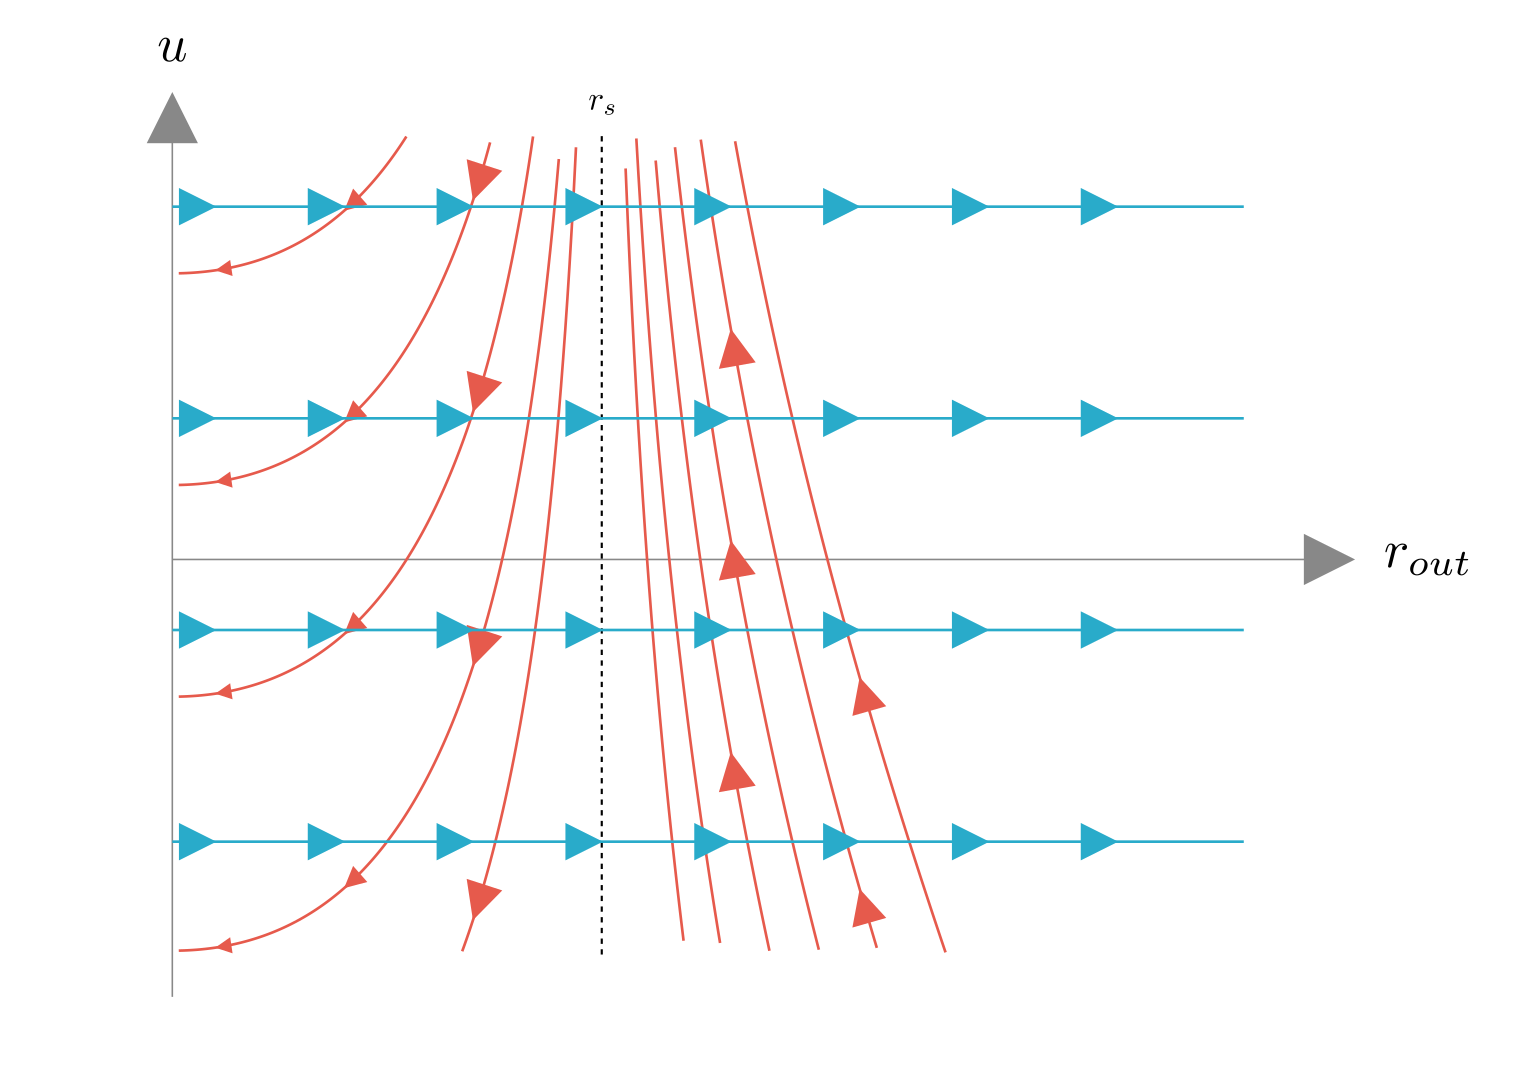
\includegraphics[width=\linewidth]{AgujerosNegros/Schwarzschild/media/images/EddingtonFinkelsteinUR_ManimCE_v0.19.0.png} 
        \caption{Rayos de luz en coordenadas de Eddington-Finkelstein salientes.}
    \end{subfigure}
    \caption{Se muestra la gráfica de los rayos de luz en coordenadas avanzadas y las nuevas coordenadas no ortogonales que están definidas como $u = ct - r - r_s \log \left| \frac{r}{r_s} - 1 \right|, \quad r_{\text{out}} = r$.}
\end{figure}

\subsubsection{Métrica en coordenadas salientes}
El calculo en coordenadas salientes se realiza de manera análoga al caso entrante.
\begin{equation}
    \begin{aligned}
        \v{e_u   }             & = \frac{\partial ct}{\partial u} \v{e_{ct}} + \frac{\partial r}{\partial u} \v{e_r} = \v{e_{ct}},                                                             \\
        \v{e_{r_{\text{out}}}} & = \frac{\partial ct}{\partial r_{\text{out}}} \v{e_{ct}} + \frac{\partial r}{\partial r_{\text{out}}} \v{e_r} = \frac{1}{1 - \frac{r_s}{r}} \v{e_{ct}} + \v{e_r}.
    \end{aligned}
\end{equation}

Componentes de la métrica \( g_{\mu\nu} = \v{e_\mu} \cdot \v{e_\nu} \):
\begin{equation}
    \begin{aligned}
        g_{uu}          & = \v{e_u} \cdot \v{e_u} = -\left(1 - \frac{r_s}{r}\right), \\
        g_{ur} = g_{ru} & = \v{e_u} \cdot \v{e_{r_{\text{out}}}} = -1,               \\
        g_{rr}          & = \v{e_{r_{\text{out}}}} \cdot \v{e_{r_{\text{out}}}} = 0.
    \end{aligned}
\end{equation}

La métrica en coordenadas salientes es:
\begin{equation}
    ds^2 = -\left(1 - \frac{r_s}{r}\right) du^2 - 2 du dr + r^2 d\Omega^2.
\end{equation}

\subsubsection{Propiedades de las coordenadas de Eddington-Finkelstein}
El cambio de coordenadas permite mostrar que las partículas de luz/masivas puedan pasar a través del horizonte de eventos, pero...
\begin{itemize}
    \item En coordenadas de EF entrantes: los haces de luz salientes no funcionan en $r_s$.
    \item En coordenadas de EF salientes: los haces de luz entrantes no funcionan en $r_s$.
\end{itemize}


\subsection{Coordenadas Kruskal-Szekeres}
La idea detrás de las coordenadas Kruskal-Szekeres es extender las coordenadas de Eddington-Finkelstein manteniendo los rayos de luz salientes y entrantes con pendiente $\pm 1$ obteniendo las ventajas de los diagramas de coordenadas avanzadas y retrasadas, en uno solo.

Se usa la ventaja de montar los vectores base sobre los rayos de luz entrantes y salientes, y se define un nuevo conjunto de coordenadas \( (U, V) \) que son funciones de las coordenadas de Eddington-Finkelstein \( (u, v) \).
\subsubsection{Coordenadas nulas originales}
Con las coordenadas entrante (\(v\)) y saliente (\(u\)) de Eddington-Finkelstein que usan en conjunto la parte espacial y temporal original
\begin{equation}
    \begin{aligned}
        v   & = ct + r^*                                      \\
        u   & = ct - r^*                                      \\
        r^* & \equiv r + r_s \log\left|\frac{r}{r_s}-1\right|
    \end{aligned}
\end{equation}
se puede recobrar las componentes temporal y espacial \( (r, ct) \) como 
\begin{equation}
\frac{v+ u}{2} = ct, \quad \frac{v- u}{2} = r^*.
\label{eq:ryt_in_terms_of_uv}
\end{equation}


\subsubsection{Vectores base en coordenadas \( (u, v) \)}
Expresamos los vectores base en términos de \( e_{ct} \) y \( e_r \):
\begin{equation}
    \begin{aligned}
        \v{e_v} & = \frac{\partial ct}{\partial v}\v{e_{ct}} + \frac{\partial r}{\partial v}\v{e_r} = \frac{1}{2}\v{e_{ct}} + \frac{1}{2}\left(1-\frac{r_s}{r}\right)\v{e_r} \\
        \v{e_u} & = \frac{\partial ct}{\partial u}\v{e_{ct}} + \frac{\partial r}{\partial u}\v{e_r} = \frac{1}{2}\v{e_{ct}} - \frac{1}{2}\left(1-\frac{r_s}{r}\right)\v{e_r}
    \end{aligned}
\end{equation}



\subsubsection{Métrica en coordenadas nulas}

Usando la métrica de Schwarzschild \( g(e_{ct},e_{ct}) = -\left(1-\frac{r_s}{r}\right) \) y \( g(e_r,e_r) = \left(1-\frac{r_s}{r}\right)^{-1} \), se calcula los productos internos de las nuevas bases
\begin{equation}
    \begin{aligned}
       \v{ e_v }\cdot \v{e_v} & = \left(\frac{1}{2}\right)^2 g(e_{ct},e_{ct}) + \left(\frac{1}{2}\left(1-\frac{r_s}{r}\right)\right)^2 g(e_r,e_r) = 0                                        \\
        \v{ e_u }\cdot \v{e_u} & = \left(\frac{1}{2}\right)^2 g(e_{ct},e_{ct}) + \left(\frac{1}{2}\left(1-\frac{r_s}{r}\right)\right)^2 g(e_r,e_r) = 0                                        \\
        \v{ e_v }\cdot \v{e_u} & = \left(\frac{1}{2}\right)^2 g(e_{ct},e_{ct}) - \left(\frac{1}{2}\left(1-\frac{r_s}{r}\right)\right)^2 g(e_r,e_r) = -\frac{1}{2}\left(1-\frac{r_s}{r}\right).
    \end{aligned}
\end{equation}
% -------------------
\begin{figure}[H]
    \begin{small}
        \begin{center}
            \begin{otherlanguage}{english}
\begin{tikzpicture}[scale=1.2,>=Latex, line cap=round, line join=round, thin]

% Definir tamaños
\def\AxisLen{3.2}      % longitud de los ejes
\def\ConeScale{2.0}    % tamaño del cono de luz

% --- Ejes (r*, ct)
\draw[thick,->] (-0.9*\AxisLen,0) -- (\AxisLen,0) node [above]{$r^*$};
\draw[thick,->] (0,0) -- (0,\AxisLen) node [above left]{$c\,t$};

% --- Cono de luz
\begin{scope}
  \clip (-\ConeScale,0) rectangle (\ConeScale,\ConeScale);
  % Sombra / volumen del cono
  \shade [top color=yellow!20, bottom color=orange!30, opacity=0.4] 
    (0,0) -- (\ConeScale,\ConeScale) -- (-\ConeScale,\ConeScale) -- cycle;
  
  % Bordes del cono
  \draw [thick, dashed, orange!80!red] (-\ConeScale,\ConeScale) -- (0,0) -- (\ConeScale,\ConeScale);
\end{scope}

% --- Flechas de la base original
\draw[->, thick, cyan!70!black] (0,0) -- (0,1.8) node [above right]{$e_{ct}$};
\draw[->, thick, cyan!70!black] (0,0) -- (1.8,0) node [above right]{$e_r$};

% --- Flechas de la nueva base (combinación)
\draw[->, thick, magenta!80!black] (0,0) -- (1.4,1.4) node [ right]{$e_v$};
\draw[->, thick, magenta!80!black] (0,0) -- (-1.4,1.4) node [ left]{$e_u$};

\end{tikzpicture}
\end{otherlanguage}
        \end{center}
        \caption{Los nuevos vectores base $\v{e_u}$ y $\v{e_v}$ de tipo nulo están en direcciones tipo luz y son una composición de los vectores base originales.}
    \end{small}
\end{figure}
El uso directo de ambas coordenadas tipo luz entrantes y salientes de Eddington-Finkelstein aun presenta un problema en $r_s$ y es que $\v{e_v}\cdot \v{e_u}$ se solapan y la métrica  
\begin{equation}
    ds^2 = 2(e_v \cdot e_u) du\, dv + r^2 d\Omega^2 = -\left(1-\frac{r_s}{r}\right) du\, dv + r^2(d\theta^2 + \sin^2\theta d\varphi^2),
\end{equation}
en su parte $g_{uv}$ se vuelve cero.


\subsubsection{Transformación a Kruskal-Szekeres}
El problema de querer usar ambas coordenadas de Eddington-Finkelstein se puede rastrear al logaritmo tal que para deshacernos de el 

\begin{equation}
    \begin{aligned}
        \frac{v-u}{2}&=r+r_s \log \left|\frac{r}{r_s}-1\right|                 \\
        \frac{v-u}{2 r_s}&=\frac{r}{r_s}+\log \left|\frac{r}{r_s}-1\right|     \\
        e^{\frac{v-u}{2 r_s}}&=e^{\frac{r}{r_s}+\log \abs{ \frac{r}{r_s} - 1} }, \\
        -e^{\frac{v}{2 r_s}}\left(-e^{-\frac{u}{2 r_s}}\right)&=e^{\frac{r}{r_s}}\left|\frac{r}{r_s}-1\right|
    \end{aligned}
\end{equation}
(La razón de poner $-e(-e)$ es meramente a conveniencia para que las nuevas coordenadas sean escalaciones de $\v{e_v}$ y $\v{e_u}$).
Definimos las nuevas coordenadas
\begin{equation}
    U = -e^{-\frac{u}{2r_s}}, \quad V = e^{\frac{v}{2 r_s}}
\end{equation}

Los vectores base en Kruskal-Szekeres 
\begin{equation}
    \begin{aligned}
        \v{e_U} & = \frac{\partial u}{\partial U} \v{e_u} = 2r_s e^{\frac{u}{2r_s}} \v{e_u}  = 2r_s U^{-1} \v{e_u} \\
        \v{e_V} & = \frac{\partial v}{\partial V} \v{e_v} = -  2r_s \left(- e^{-\frac{v}{2r_s}}\right) \v{e_v} =- 2r_s V^{-1} \v{e_v}
    \end{aligned}
\end{equation}

\subsubsection{Métrica de Kruskal-Szekeres}
Calculamos el producto punto usando \( \v{e_u} \cdot \v{e_v} = -\frac{1}{2}\left(1-\frac{r_s}{r}\right) \)
\begin{equation}
    \v{e_U} \cdot \v{e_V} = (2r_s U^{-1})(-2r_s V^{-1})(\v{e_u} \cdot \v{e_v}) = - \frac{2r_s^2}{U V}\left(1-\frac{r_s}{r}\right)
\end{equation}

De la definición de \( U \) y \( V \) se obtiene $UV = -e^{\frac{r}{r_s}}\left|\frac{r}{r_s} - 1\right|$ para sustituirlo en el producto punto
\begin{equation}
    \begin{aligned}
        \v{e_U} \cdot \v{e_V} &= (2r_s U^{-1})(-2r_s V^{-1})(\v{e_u} \cdot \v{e_v}) = \frac{2r_s^2 e^{-\frac{r}{r_s}}}{\left(\frac{r}{r_s} - 1\right)}\left(1-\frac{r_s}{r}\right)\\
        & =2r_s^2 e^{-\frac{r}{r_s}} \frac{\left(\frac{r - r_s}{r}\right)}{\left(\frac{r -r_s}{r_s}\right)}\\
        & = \frac{2r_s^3}{r} e^{-\frac{r}{r_s}}.
    \end{aligned}
\end{equation}

La métrica toma su forma canónica:
\begin{equation}
    ds^2 = \frac{2 r_s^3}{r}e^{-\frac{r}{r_s}} dUdV + r^2(d\theta^2 + \sin^2\theta d\varphi^2).
\end{equation}

De momento $V$ y $U$ son coordenadas nulas, que describen trayectorias de luz, ya que estas son escalaciones de $u,v$ podemos hacer un análogo a la ecuación \ref{eq:ryt_in_terms_of_uv} para definir coordenadas espacial y temporal 
\begin{equation}
    \begin{aligned}
        T \equiv \frac{V+U}{2} \\
        X \equiv \frac{V-U}{2} \\
    \end{aligned}
\end{equation}
y viceversa
\begin{equation}
    \begin{aligned}
        V=T+X \\
        U=T-X
    \end{aligned}
\end{equation}
De modo que la métrica en términos de $T$ y $X$ es:
\begin{equation}
        g_{\mu \nu} =\left[\begin{array}{cccc}
                                             +\frac{4 r_s^3}{r} e^{-\frac{r}{r_s}} & 0                                     & 0    & 0                   \\
                                             0                                     & -\frac{4 r_s^3}{r} e^{-\frac{r}{r_s}} & 0    & 0                   \\
                                             0                                     & 0                                     & -r^2 & 0                   \\
                                             0                                     & 0                                     & 0    & -r^2(\sin \theta)^2
                                         \end{array}\right]
\end{equation}
Usando $ds^2 = 0 $ encontramos las geodésicas nulas en estas coordenadas
\begin{equation}
    \begin{array}{l}
        
        0=\left(\frac{d T}{d \lambda}\right)^2 g_{T T}+\left(\frac{d X}{d \lambda}\right)^2 g_{X X}                                                                                                                                     \\
        0=\left(\frac{d T}{d \lambda}\right)^2\left(+2 g_{U V}\right)+\left(\frac{d X}{d \lambda}\right)^2\left(-2 g_{U V}\right)
    \end{array}
\end{equation}

\begin{equation}
    \d{X}{\lambda} =\pm \d{T}{\lambda} \to \d{X}{T} = \pm 1 \to T = \pm Y + k.
\end{equation}
Eso quiere decir que las geodésicas nulas en estas coordenadas son rectas en el espacio-tiempo. 
ahora volver a poner las coordenadas en términos de $r$ y $t$ solo es cuestión de una composición de funciones.

\begin{equation}
    \begin{aligned}
        T&=\frac{V+U}{2} \\
        X&=\frac{V-U}{2}
    \end{aligned}
    \quad ; 
    \begin{aligned}
        V&=e^{\frac{v}{2 r_s}} \\
        U&=-e^{-\frac{u}{2 r_s}}
    \end{aligned}
    \quad ; 
    \begin{aligned}
        v&=c t+r+r_s \log \left|\frac{r}{r_s}-1\right| \\
        u&=c t-r-r_s \log \left|\frac{r}{r_s}-1\right|
    \end{aligned}
\end{equation}
Simplificando
\begin{equation}
    \begin{aligned}
        T & =  \frac{1}{2}\left(V + U\right)                                                                                                                                                      \\
          & = \frac{1}{2} e^{\frac{v}{2 r_s}}-\frac{1}{2} e^{-\frac{u}{2 r_S}}                                                                                                                    \\
          & = \frac{1}{2} e^{\frac{1}{2 r_s}\left(c t+r+r_s \log \left|\frac{r}{r_s}-1\right|\right)}-\frac{1}{2} e^{-\frac{1}{2 r_s}\left(c t-r-r_s \log \left|\frac{r}{r_s}-1\right|\right)}    \\
          & =\frac{1}{2} e^{\frac{c t}{2 r_s}} e^{\frac{r}{2 r_s}}\left(\left|\frac{r}{r_s}-1\right|\right)^{1 / 2}-\frac{1}{2} e^{\frac{-c t}{2 r_s}} e^{\frac{r}{2 r_s}}\left(\left|\frac{r}{r_s}-1\right|\right)^{1 / 2} \\
          & = e^{\frac{r}{2 r_s}} \sqrt{\left|\frac{r}{r_s}-1\right|} \frac{1}{2}\left(e^{\frac{c t}{2 r_s}}-e^{\frac{-c t}{2 r_s}}\right)                                                                     \\
          & = e^{\frac{r}{2 r_s}} \sqrt{\left|\frac{r}{r_s}-1\right|} \sinh\left(\frac{ct}{2r_s}\right)
          \label{eq:Kruskal-SzekeresT(r,t)}
    \end{aligned}
\end{equation}
y para $X$ el calculo es prácticamente el mismo a excepción de un signo ($+$) en la diferencia de exponentes.
\begin{equation}
        X  = e^{\frac{r}{2 r_s}} \sqrt{\left|\frac{r}{r_s}-1\right|}  \cosh\left(\frac{ct}{2r_s}\right)
        \label{eq:Kruskal-SzekeresX(r,t)}
\end{equation}
Donde podemos desarrollar la siguiente identidad
\begin{equation}
    \begin{aligned}
         X^2 -T^2  &=  \left( e^{\frac{r}{2r_s}} \sqrt{\left|\frac{r}{r_s}-1\right|}\, \cosh\left(\frac{ct}{2r_s}\right) \right)^2- \left( e^{\frac{r}{2r_s}} \sqrt{\left|\frac{r}{r_s}-1\right|}\, \sinh\left(\frac{ct}{2r_s}\right) \right)^2 \\[1mm]
        &= e^{\frac{r}{r_s}} \left|\frac{r}{r_s}-1\right| \left[ \cosh^2\left(\frac{ct}{2r_s}\right) -\sinh^2\left(\frac{ct}{2r_s}\right) \right]\\[1mm]
        &= \, e^{\frac{r}{r_s}} \left|\frac{r}{r_s}-1\right|\\[2mm]
        &=
        \begin{cases}
            \, e^{\frac{r}{r_s}} \left(\dfrac{r}{r_s}-1\right), & \text{si } r > r_s,\\[2mm]
            \, e^{\frac{r}{r_s}} \left(1-\dfrac{r}{r_s}\right), & \text{si } r < r_s.
        \end{cases}
    \end{aligned}
    \label{eq:Kruskal-SzekeresT^2-X^2}
\end{equation}

\noindent
Esta identidad nos ayuda a determinar las líneas de \(r\) constante en el espacio-tiempo de Schwarzschild. Lo interesante ocurre cuando observamos el caso \(r < r_s\): el valor absoluto \(\left|\frac{r}{r_s}-1\right|\) en la ecuación (\ref{eq:Kruskal-SzekeresT^2-X^2}) se puede expresar como \(1-\frac{r}{r_s}\). ¿Por qué es importante notar esto? Si nos fijamos en la segunda línea de la ecuación, podemos identificar los coeficientes de la siguiente forma:
\begin{equation}
    \begin{aligned}
       X^2 -  T^2  &= e^{\frac{r}{r_s}} \left(1-\frac{r}{r_s}\right) \left[ \cosh^2\left(\frac{ct}{2r_s}\right) - \sinh^2\left(\frac{ct}{2r_s}\right) \right] \\
        &= -\, e^{\frac{r}{r_s}} \left(\frac{r}{r_s}-1\right) \left[ \cosh^2\left(\frac{ct}{2r_s}\right) - \sinh^2\left(\frac{ct}{2r_s}\right) \right] \\
        &= e^{\frac{r}{r_s}} \left(\frac{r}{r_s}-1\right) \left[ \sinh^2\left(\frac{ct}{2r_s}\right) - \cosh^2\left(\frac{ct}{2r_s}\right) \right].
    \end{aligned}
\end{equation}
De ello se deduce que, dentro del horizonte de eventos (\(r < r_s\)), se tienen las siguientes expresiones:
\begin{equation}
    X = e^{\frac{r}{2r_s}} \sqrt{\frac{r}{r_s}-1} \, \frac{1}{2} \sinh\left(\frac{ct}{2r_s}\right), \quad 
    T = e^{\frac{r}{2r_s}} \sqrt{\frac{r}{r_s}-1} \, \frac{1}{2} \cosh\left(\frac{ct}{2r_s}\right).
\end{equation}
Esto implica que, dentro del horizonte de eventos, las coordenadas \(T\) y \(X\) se invierten en comparación con el caso fuera del horizonte. Dado este intercambio de coordenadas cuando se pasa el horizonte de eventos, normalmente por conveniencia matemática la ecuación \ref{eq:Kruskal-SzekeresT^2-X^2} se expresa sin el valor absoluto, es decir:
\begin{equation}
    X^2 - T^2 = e^{\frac{r}{r_s}} \left(\frac{r}{r_s}-1\right) \left[ \cosh^2\left(\frac{ct}{2r_s}\right) - \sinh^2\left(\frac{ct}{2r_s}\right) \right],
\end{equation} 
para $r \, \epsilon \, [0,\infty ) $.

Dado que el negativo de estas coordenadas $-X$ y $-T$ cumplen la identidad (\ref{eq:Kruskal-SzekeresT^2-X^2}) podemos escribir lo que se llama la extensión máxima de las coordenadas de Kruskal-Szekeres
\begin{table}[H]
    \centering
    \caption{Extensión máxima de las coordenadas de Kruskal-Szekeres}
    \begin{tabular}{|c|c|c|}
        \hline Region & $T$                                                                                         & $X$                                                                                \\
        \hline$I$        & $+\sinh \left(\frac{c t}{2 r_s}\right)\frac{r}{2 r_s} \sqrt{\frac{r}{r_s}-1}$ & $+\cosh \left(\frac{c t}{2 r_s}\right) e^{\frac{r}{2 r_s}} \sqrt{\frac{r}{r_s}-1}$ \\
        \hline$I I$       & $+\cosh \left(\frac{c t}{2 r_s}\right) e^{\frac{r}{2 r_s}} \sqrt{1-\frac{r}{r_s}}$          & $+\sinh \left(\frac{c t}{2 r_s}\right) e^{\frac{r}{2 r_s}} \sqrt{1-\frac{r}{r_s}}$ \\
        \hline$I I I$   & $-\sinh \left(\frac{c t}{2 r_s}\right) e^{\frac{r}{2 r_s}} \sqrt{\frac{r}{r_s}-1}$          & $-\cosh \left(\frac{c t}{2 r_s}\right) e^{\frac{r}{2 r_s}} \sqrt{\frac{r}{r_s}-1}$ \\
        \hline$I V$      & $-\cosh \left(\frac{c t}{2 r_s}\right) e^{\frac{r}{2 r_s}} \sqrt{1-\frac{r}{r_s}}$          & $-\sinh \left(\frac{c t}{2 r_s}\right) e^{\frac{r}{2 r_s}} \sqrt{1-\frac{r}{r_s}}$ \\
        \hline
    \end{tabular}
\end{table}

\noindent Ahora para la lineas de tiempo constante es fácil ver la siguiente relación
\begin{equation}
    \tanh \left(\frac{ct}{2 r_s}\right)=\left\{\begin{array}{ll}
        T / X & \text { (en region I y III) } \\
        X / T & \text { (en region II y IV) }
        \end{array}\right.
\end{equation}
Con esto tenemos todo lo necesario para construir el diagrama de Kruskal-Szekeres.  
\begin{figure}[H]
    \begin{small}
        \begin{center}
            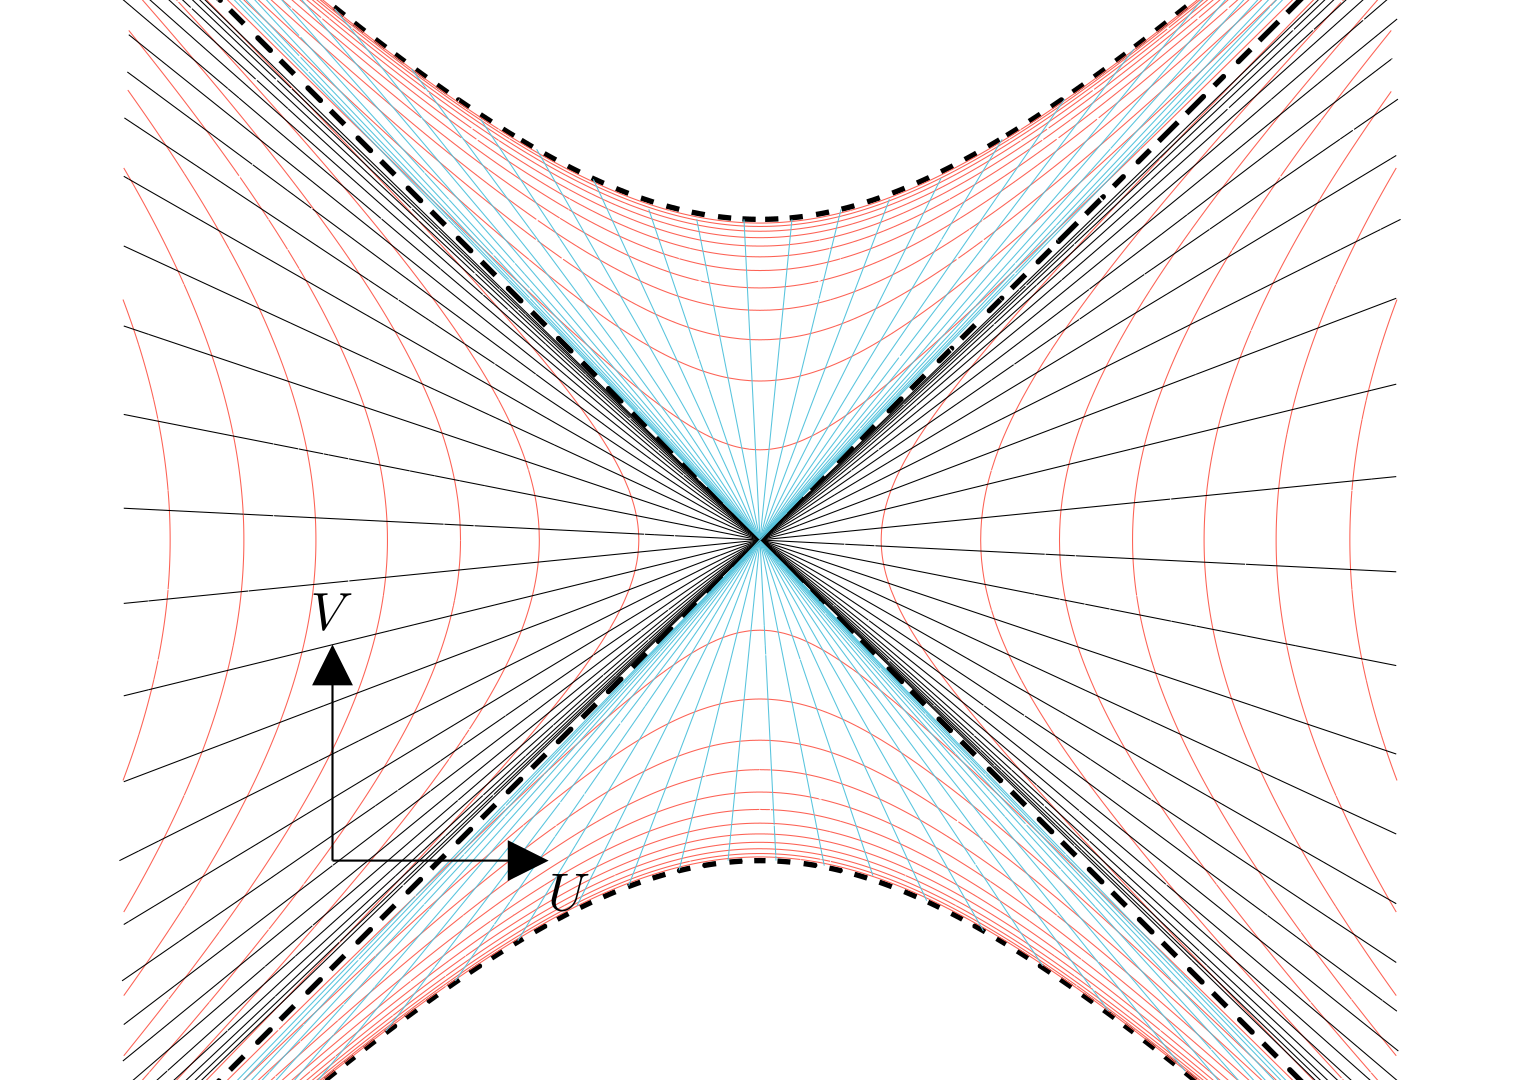
\includegraphics[width=0.95\textwidth]{AgujerosNegros/Schwarzschild/media/images/Kruskal_Szekeres_diagram_ManimCE_v0.19.0.png}
        \end{center}
        \caption{El diagrama de Kruskal-Szekeres muestra las líneas de luz (en azul) y las líneas de tiempo (en rojo) en las coordenadas \(T\) y \(X\). Las líneas de luz tienen pendiente \(\pm 1\), lo que indica que la velocidad de la luz es constante en todas las direcciones. El horizonte de eventos está representado por las líneas diagonales que separan las regiones I, II, III y IV.}
        \label{fig:Kruskal_Szekeres_diagram}
    \end{small}
\end{figure}
En la figura \ref{fig:Kruskal_Szekeres_diagram} los conos de luz tienen pendiente \(\pm 1\) .




